% Created 2015-04-20 lun. 15:27
\documentclass[a4paper]{article}
\usepackage[french]{babel}
\usepackage[utf8]{inputenc}
\usepackage[T1]{fontenc}
\usepackage{hyperref}
\usepackage{graphicx}
\tolerance=1000
\usepackage{indentfirst}
\usepackage[top=4cm,bottom=4cm,right=4cm,left=4cm]{geometry}
\author{Emery, Gouraud, Kirov, Pouteau}
\date{Mercredi 22 Avril 2015}
\title{\textbf{RAPPORT PROJET 2048}}
\hypersetup{
  pdfkeywords={},
  pdfsubject={},
  pdfcreator={Emacs 24.4.1 (Org mode 8.2.10)}}
 \begin{document}

 \maketitle
 \tableofcontents

 \newpage
 \section{Introduction}
 \label{sec-1}

 Dans le cadre de l'UE Environnement de Développement et Projet de
 Programmation 1, nous avons été amené à créer un jeu 2048.\\
 Ce jeu consiste à obtenir une tuile de valeur 2048 en fusionnant des
 tuiles de même valeur de manière à en obtenir une deux fois plus
 grande. Le jeu commence avec deux tuiles de valeur aléatoire (2 ou 4). Il se joue
 sur une grille de 4x4, avec quatre déplacements possibles (Haut, Bas, Droite, Gauche). 
 A chaque déplacement une tuile de valeur 2 ou 4 apparait aléatoirement sur la grille.\\
 Ce jeu est une application mobile sortie en mars 2014, programmé par
 Gabriele Circulli, un web-designer italien. Il s'est inspiré du jeu
 1024 dont le principe est identique sauf le but qui est
 d'atteindre pour le coup 1024. Ce jeu 1024 est lui-même basé sur Threes un jeu du
 même style.

 \noindent
 Lien pour tester les différents jeux: 

 \begin{itemize}
 \item lien 2048: \url{http://gabrielecirulli.github.io/2048/}

 \item lien 1024: \url{http://1024game.org}

 \item lien Threes: \url{http://threesjs.com}
 \end{itemize}

 \vspace{1cm}
 \noindent
 Le projet a été séparé en deux parties différentes.
 \begin{itemize}
 \item Réalisation de l'implémentation du 2048 et création d'une interface
 graphique sur le terminal.
 \item Réalisation d'une interface graphique indépendante et conception de
 deux IA capables de résoudre le 2048.
 \end{itemize}


 \newpage

 \section{Architecture du Projet}
 \label{sec-2}

 On a choisi une architecture classique pour notre projet.
 \begin{itemize}
 \item Un dossier include/ pour toutes les interfaces
 \item Un dossier src/ contenant
 \begin{itemize}
 \item Un dossier grid/ contenant les implémentations du jeu général
 \item Un dossier ncurses/ contenant l'implémentation de l'interface du terminal
 \item Un dossier sdl/ contenant l'implémentation de l'interface graphique et les différentes images nécessaires.
 \item Un dossier strategy/ contenant nos deux stratégies fast/low et différentes implémentations pour observer le 
 déroulement des Intelligences Artificielles.
 \item Un dossier test-fonction/ contenant l'implémentation des tests
 \end{itemize}
 \end{itemize}


 \hyperref[sec-7-1]{cf: Annexe 1 - Architecture Projet}
 \newpage
 \section{Implémentation du 2048}
 \label{sec-3}
 \subsection{Fonction de Base}
 \label{sec-3-1}
 Implémentation des fonctions décrites dans l'interface fournis
 \emph{grid.h}.

 \begin{verbatim}
 /* Créer une nouvelle grille */
 grid new_grid ();

 /* Supprime la grille passée en paramètre*/
 void delete_grid (grid g); 

 /* Copie une grille src dans une grille dst */
 void copy_grid (grid src, grid dst);

 /* Renvoie le score actuel du jeu */
 unsigned long int grid_score (grid g);

 /* Renvoie la valeur d'une tuile */ 
 tile get_tile (grid g, int x, int y); 

 /* Met la valeur t dans une tuile  */
 void set_tile (grid g, int x, int y, tile t);

 /* Verifie que la direction 'd' est valide */ 
 bool can_move (grid g, dir d); 

 /* Renvoie game_over si il n'y a plus de déplacement possible */
 bool game_over (grid g);

 /* Effectue un mouvement selon la direction 'd' */
 void do_move (grid g, dir d);

 /* Ajoute une tuile aléatoirement de valeur 2 ou 4 sur la grille. */
 void add_tile (grid g); 

 /* Effectue le mouvement et ajoute une tuile */
 void play (grid g, dir d);
 \end{verbatim}

 \vspace{0.5cm}
 Ces fonctions permettent le bon fonctionnement du jeu.  
 Nous avons essayé de simplifier toutes ces fonctions de bases. Pour
 cela, et afin d'éviter des duplications de code notamment dans
 \texttt{can\_move} et \texttt{do\_move}, nous avons fait appel à des fonctions static.

 \newpage
 \subsection{Fonction static}
 \label{sec-3-2}
 \noindent
 \underline{Déclaration des fonctions static de grid.c}:
 \begin{verbatim}
 /* Permet d'incrementer deux variables ayant 
   des incrementations differentes. */

 static void 
 incrementation(int *i1, int *i2, 
                int incrementationI1, 
                int incrementationI2)

 /*
  * Déplace l'ensemble de la grille dans la direction voulue 
  * Les directions prérequis: 
  *    UP    -> (grid, 0, 0, 0, 1)
  *    DOWN  -> (grid, 0, GRID_SIDE - 1, 0, -1)
  *    LEFT  -> (grid, 0, 0, 1, 0)
  *    RIGHT -> (grid, GRID_SIDE - 1, 0, -1, 0)
  */
 static void move(grid g, int i, int j, int a, int b);

 /*
  * Teste sur l'ensemble de la grille si le deplacement
  * dans la direction voulue est faisable
  * (en fonction des paramètres) 
  * Les directions prérequis :  
  *    UP    -> (grid, 0, 0, 0, 1)
  *    DOWN  -> (grid, 0, GRID_SIDE - 1, 0, -1)
  *    LEFT  -> (grid, 0, 0, 1, 0)
  *    RIGHT -> (grid, GRID_SIDE - 1, 0, -1, 0)
  */
 static bool possible(grid g, int i, int j, int a, int b);

 /* Fusionne deux cases et met la deuxième case à 0 */
 static void fusion(grid g, int i, int j, int a, int b);

 /* Ajoute add_score au score de la grid */
 static void set_grid_score(grid g, unsigned long int add_score);
 \end{verbatim}

 \bigskip
 \underline{Description de l'utilisation des fonctions static}: 
 \begin{itemize}
 \item \textbf{move} :
 Elle sert à simplifier la fonction \texttt{do\_move}, car elle effectue tous 
 les déplacements en fonction des paramètres fournis. Par conséquent,
 \texttt{do\_move} est reduite à appeler simplement \texttt{move} avec les bons paramètre.
 \item \textbf{fusion} :
 Elle est utilisée pour faire les fusions dans la fonction \texttt{move}.
 \item \textbf{incrementation} :
 Elle permet d'éviter la répétition de code due à l'incrémentation des
 variables dans \texttt{move} et \texttt{possible}.
 \item \textbf{possible} : 
 Elle permet de simplifier la fonction \texttt{can\_move}, car lorsqu'on lui passe
 certains paramètres, elle vérifie la possibilité de faire un
 mouvement. Ce qui réduit la fonction \texttt{can\_move} à appeler la
 fonction \texttt{possible} avec les bons paramètres.
 \end{itemize}
 \newpage
 \subsection{Réalisation de test}
 \label{sec-3-3}

 Les tests sont déclenchés par la commande \textbf{make check}.
 \bigskip\\
 Nous avons utilisé gcov, ce qui nous a permis de savoir que notre
 programme de test vérifie 94.96\% de notre fichier grid.c.
 Les 5\% manquant sont dus au fait que l'on ne teste pas la fonction
 \texttt{play} car elle utilise simplement deux autres fonctions testées précédemment.

 \begin{verbatim}
 File 'grid.c'
 Ligne exécutées: 94.96% de 139
 Creating 'grid.c.gcov'
 \end{verbatim}
 \noindent
 Nous avons testé indépendamment chaque déplacement, pour savoir
 précisément quel déplacement pourrait provoquer une erreur. 


 Les tests ont été réalisé de manière à être extensible c'est-à-dire
 que quelque soit la valeur de \texttt{GRID\_SIDE} les tests permettent de
 tester les différentes fonctions.

 \hyperref[sec-7-2]{cf: Annexe 2 - Execution des tests}
 \newpage
 \section{Interface Graphique}
 \label{sec-4}
 \subsection{Interface Graphique sur terminal}
 \label{sec-4-1}

 Nous avons choisi d'utiliser la bibliothèque Ncurses pour pouvoir
 générer notre grille dans le terminal.\\
 Le jeu se joue avec les flèches directionnelles. Nous avons intégré
 des couleurs afin d'égayer l'affichage de notre jeu.\\
 Nous proposons également des options supplémentaires:
 \begin{itemize}
 \item q: permet de quitter le jeu
 \item r: permet de recommencer le jeu
 \end{itemize}
 De plus, si vous perdez, on vous offre la possibilité de soit rejouer,
 soit quitter le jeu.\\
 Nous avons également intégré, par esprit de challenge, un Highscore. \\
 L'affichage graphique s'adapte à la taille de la grille. Mais ne
 modifie pas la taille du terminal d'où il est lancé.

 \subsection{Interface Graphique SDL}
 \label{sec-4-2}

 A partir de la bibliothèque SDL et de ses bibliothèques tierces (\texttt{SDL\_image}, 
 \texttt{SDL\_ttf} et \texttt{SDL\_getenv}), nous avons créé l'interface graphique du 2048 sur 
 une fenêtre indépendante. Cette fenêtre s'ouvre centrée à l'écran, et s'adapte
 à la taille de la grille (\texttt{GRID\_SIDE}) définit dans le grid.h.
 Le texte apparait parfaitement centré et est inhérent à \texttt{GRID\_SIDE}. La police
 du texte est aussi en adéquation avec la taille de la grille.\\
 L'interface graphique propose aussi de recommencer la partie (touche "Entrée"),
 mais aussi d'abandonner (touche "Echap" ou la croix en haut à droite) et ferme 
 le programme.\\
 Lorsque la partie se termine (c'est-à-dire lorsqu'aucun déplacement n'est possible),
 le joueur (s'il a obtenu un nouvel Highscore) a la possibilité de mémoriser son 
 pseudo. S'il n'entre pas son pseudo (par exemple : en relançant la partie ou en quittant le programme),
 le pseudo qui sera mis par défaut sera "Anyone".\\
 Le code est commenté de façon à être compréhensible et le nom des variables
 est en anglais.\\
 Il n'y a aucune fuite de mémoire, mis à part celle de base liée à la
 SDL et référencée.
 \vspace{0.2cm}
 \noindent
 Nous avons intégré des options supplémentaires. Le jeu se lance sur un
 menu qui permet de choisir le dégradé des tuiles du jeu. De plus, nous
 pouvons égalemment changer la couleur grâce aux touches "F1" "F2" et "F3" durant la partie.
 Cela n'est pas clairement précisé, car il s'agit en faite d'un Easter Egg.\\
 Nous avons pour finir, intégré une petite animation dans le menu du jeu.
 Pour illustrer le tout, voici un screenshot du menu :\\
 \hyperref[sec-7-3]{Annexe 3 - Image menu jeu sdl}

 \newpage
 \section{Intelligence Artificielle}
 \label{sec-5}

 Nous avons implémenté deux Intelligences Artificielles, une qui doit
 réalisé le meilleur score en moins de 10 secondes et une autre en moins de 2
 minutes.

 Pour observer nos Intelligence Artificielle à l'oeuvre nous avons
 conçu deux programmes de visualisation. La première permettant de
 répeter \emph{n} fois l'Intelligence Artificielle et une autre permettant
 de l'observer grâce à un affichage Ncurses, un mouvement est fait à
 chaque fois que l'on presse la touche "UP".


 Les résultats des différentes Intelligence Artificielle sur 100 lancés sont disponibles en annexe 3.\\
 \hyperref[sec-7-4]{cf: Annexe 4 - Intelligence Artificielle}

 \vspace{0.2cm}
 \noindent
 \underline{Le principe de notre fonction d'exploration}:\\
 Elle crée un tableau de 4 cases permettant de stocker les scores issus
 des 4 directions. Si la profondeur est de 0 alors elle renvoie la note
 de la grille en cours. Tout d'abord, la fonction effectue un mouvement
 dans une direction à la profondeur \emph{n}, puis elle génère l'apparition de 
 la tuile 2 sur une case vide de la grille et la fonction se rappelle 
 avec une profondeur de \emph{n-1}. Elle fait de même avec l'apparition d'un 4 
 sur la même case vide. Elle effectue cette série d'opérations sur toutes 
 les cases vides de la grille courante. Une fois qu'elle a parcouru toutes 
 les cases vides, elle calcule la moyenne des notes obtenues. Elle la stock 
 alors dans la case du tableau correspondant à la direction effectuée. 
 Elle choisie ensuite la meilleure note parmi les 4 directions et la renvoie. 
 En parallèle, elle modifie une variable de direction passée par référence. 
 Le mouvement à effectuer est alors cette variable directionnelle.


 \subsection{Intelligence Artificielle Rapide}
 \label{sec-5-1}
 Dans l'Intelligence Artificielle Rapide, nous avons décidé de faire une 
 exploration de 2 et d'étendre à 3 lorsque qu'il ne reste que 0 ou 1 case 
 vide dans la grille.

 \noindent

 \subsection{Intelligence Artificielle Lente}
 \label{sec-5-2}
 Dans l'Intelligence Artificielle Lente, nous avons décidé de faire
 une exploration de profondeur:
 \begin{itemize}
 \item 2 par défaut
 \item 3 pour lorsque qu'il reste moins de 6 cases vides
 \item 4 pour lorsque qu'il reste moins de 3 cases vides
 \item 5 pour lorsque qu'il reste moins de 2 cases vides
 \end{itemize}

 \vspace{0.5cm}


 \newpage
 \subsection{Fonction de notation}
 \label{sec-5-3}
 \noindent
 Nous avons une fonction de note générale qui utilise une autre fonction.

 \underline{Fonction \texttt{grid\_note}}:
 \begin{verbatim}
 static long int grid_note(grid g){
   long int cpt = 0;
   int cpt_case_empty = 0;
   int cpt_sign_change = 0;
   int max = 0;
   // Parcours de la grille
   for(int y = 0; y < GRID_SIDE; y++){
     for(int x = 0; x < GRID_SIDE; x++){
       cpt += get_tile(g, x, y);
       // Determination de la valeur maximum 
       if(get_tile(g, x, y) > max)
                 max = get_tile(g, x, y);
       // Determination du nombre de case vide
       if(get_tile(g, x, y) == 0)
                 cpt_case_empty++;
       // Monotonicite de la grille 
       cpt_sign_change += monotonicity(g, x, y);
     }
     // Bonus coin superieur gauche
     if(get_tile(g, 0, 0) == max)
       cpt += BONUS_CORNER * max;
     // Autres bonus
     cpt += BONUS_HIGH_MAXIMUM * pow(2, max);
     cpt += BONUS_SCORE * grid_score(g);
     cpt += BONUS_CASE_EMPTY * cpt_case_empty;
     // Malus si pas monotone
     cpt -= MALUS_SIGN_CHANGE * cpt_sign_change;

     return cpt;
   }
 \end{verbatim}

 Notre fonction de notation \texttt{grid\_note} parcours une fois la grille et durant le parcours elle :
 \begin{itemize}
 \item détermine la somme des tuiles de la grille
 \item Récupère la valeur maximale de la grille
 \item Compte le nombre de cases vides
 \item Evalue la monotonicité de la grille grace à la fonction \texttt{monotonicity} ci-dessous
 \end{itemize}



 Ensuite la fonction attribue des \emph{bonus} et des \emph{malus} en fonction de la disposition de la grille.\\
 \underline{Bonus}:
 \begin{itemize}
 \item Si le coin en haut à gauche possède la tuile maximale
 \item Selon le nombre de cases vides (plus il y en a, mieux c'est)
 \item Selon le score
 \item Selon la tuile maximale
 \end{itemize}
 \underline{Malus}:
 \begin{itemize}
 \item Selon sa monotonicité
 \end{itemize}
 \newpage
 \noindent
 \underline{Fonction Monotonicité}:


 Nous avons besoin d'une fonction qui note la monotonicité de la grille
 c'est-à-dire nous vérifions que les grilles sont ordonnées de manière
 à ce que les meilleures soit en haut des colonnes et à gauche des lignes.
 Elle compte le nombre de cases mal ordonnées.

 \begin{verbatim}
 static long int monotonicity(grid g, int x, int y){
   int cpt_sign_change = 0;
   if(x < GRID_SIDE - 1){
     if(get_tile(g, x, y) < get_tile(g, x + 1, y))
       cpt_sign_change += get_tile(g, x + 1, y) - get_tile(g, x, y);
     if(get_tile(g, y, x) < get_tile(g, y, x + 1))
       cpt_sign_change += get_tile(g, y, x + 1) - get_tile(g, y, x);
   }  
   return cpt_sign_change;
 }
 \end{verbatim}


 \hspace{1.2cm} +$\leftarrow$\\
 +$\uparrow$
 \begin{tabular}{ | c | c | c | c | }


 \hline
 64 & 32 & 16 & 8 \\ \hline
 32 & 16 & 8  & 4 \\ \hline
 16 & 8  & 4  & 2 \\ \hline
 8  & 4  & 2  & 0 \\ \hline
 \end{tabular}


 \newpage
 \section{Oragnisation, Problème rencontré et critique}
 \label{sec-6}
 \subsection{Répartition du travail}
 \label{sec-6-1}

 Nous avons tous les quatre travaillé sur l'implémentation de grid.c
 Nous nous sommes tous entraidés lors de la réalisation de ce projet (comme pour le rapport, la correction finale des fichiers, etc.) 
 Ensuite nous nous sommes répartis le travail comme suit:

 \vspace{0.2cm}
 \noindent
 \underline{Ysabelle Emery}:
 \begin{itemize}
 \item Participation à l'implémentation de la Ncurses
 \item Réalisation des premiers tests (avant la relecture par les autres groupes)
 \item Correction des erreurs et relecture des fichiers
 \item Création de toutes les images nécessaires à l'interface graphique (tiles, boutons, sprite de l'animation, etc.)
 \item Modification de tous les tests afin de les rendre extensible à \texttt{GRID\_SIDE} (après la relecture)
 \end{itemize}
 \vspace{0.2cm}
 \underline{Jimmy Gouraud}:
 \begin{itemize}
 \item Réalisation de l'implémentation de l'interface graphique SDL
 \item Modification de la SDL afin de la rendre extensible à \texttt{GRID\_SIDE} (après la relecture)
 \item Création des commentaires et correction orthographique du projet
 \item Relecture, mise en page du page et conversion des variables en anglais
 \item Intégration d'un menu et d'une animation pour l'interface graphique
 \end{itemize}
 \vspace{0.2cm}
 \underline{Yordan Kirov}:
 \begin{itemize}
 \item Participation à la création des tests
 \item Création des commentaires
 \item Conception de différentes fonctions de notation de grille pour l'Intelligence Artificielle
 \item Pondération des différentes fonctions de notation de grille
 \item Travail sur le \LaTeX
 \end{itemize}
 \vspace{0.2cm}
 \underline{Sébastien Pouteau}:
 \begin{itemize}
 \item Création de l'interface Ncurses et modification afin de la rendre extensible (après la relecture)
 \item Factorisation de la fonction \texttt{do\_move} et \texttt{can\_move} (qui sont les fonctions finales utilisées)
 \item Conception de tous les Makefiles, de l'arborescence du projet, ainsi que de la création du dépot
 \item Réalisation des premiers tests (avant la relecture)
 \item Création de l'étude de profondeur des fonctions de l'Intelligence Artificielle
 \item Normalisation des fichiers de stratégie
 \end{itemize}
 \newpage
 \subsection{Problèmes rencontrés}
 \label{sec-6-2}
 Liste des problèmes rencontrés:
 \begin{itemize}
 \item Synchronisation entre l'équipe
 \item Utilisation des outils au début (comme svn, gdb, Makefile .. )
 \item Problème de compréhension du contrat de certaine fonction
 \item Génération des librairies dynamiques
 \end{itemize}

 \subsection{Critique des outils}
 \label{sec-6-3}
 
 \begin{itemize}
 \item GDB: Difficulté de prise en main, mais permet un débuggage efficace
 \item SVN: 
   \begin{itemize}
   \item Problème lors des commit/up sur nos machines
   \item Problème de conflit entre les versions
   \item Permet une bonne gestion d'un projet
  \item Permet d'avoir accés au ancienne version
  \end{itemize}
  
\item Doxygène: Normalisation de tous les contrats des fonctions assez fastidieux, mais produit une documentation complète.
\item \LaTeX:
  \begin{itemize}
  \item Difficulté de prise en main, d'utilisation et de compréhension
  \item Beau rendu final obtenu
  \item Simplification de l'organisation du texte
  \end{itemize}
\end{itemize}


\newpage

\section{Annexe}
\label{sec-7}
\subsection{Annexe 1 - Architecture Projet}
\label{sec-7-1}
\noindent
L'arbre du Projet:
{\footnotesize
\begin{verbatim}
Projet-Jeu 
     |                                                                                      
     + - README.txt                                             
     + - Makefile                                           
     + - include                                      
     |    |                                      
     |    + - grid.h                                      
     |    + - strategy.h                                      
     |    + - gridSDL.h                                      
     |
     + - src
          |                                           
          + - grid                                           
          |     |                                      
          |     + - Makefile                                      
          |     + - grid.c                                      
          |
          + - test-fonction                                      
          |     |                                      
          |     + - Makefile                                      
          |     + - fonction-test.c                                      
          |     + - main-fonction-test.c                                      
          |                                          
          + - ncurses
          |     |
          |     + - Makefile                                      
          |     + - main-ncurses.c                                      
          |     + - highscore_ncurses.txt                                      
          |                                           
          + - sdl
          |     |                                      
          |     + - Makefile                                      
          |     + - gridSDL.c                                      
          |     + - main-sdl.c
          |     + - arial.ttf                                      
          |     + - leadcoat.ttf                                      
          |     + - animation_penguin                                     
          |     |     + ...                               
          |     |                                      
          |     + - menu_button                                     
          |     |     + ...                               
          |     |                                      
          |     + - tiles
          |           + ...                               
          |                                           
          + - startegy
                |                                      
                + - Makefile                                      
                + - A2_emery_gouraud_kirov_pouteau_fast.c
                + - A2_emery_gouraud_kirov_pouteau_low.c
                + - main-graphique-fast.c
                + - main-repetition-fast.c
                + - main-graphique-low.c
                + - main-repetition-low.c
\end{verbatim}
}
\newpage
\subsection{Annexe 2 - Execution des tests}
\label{sec-7-2}
\noindent
Résultat de la commande \textbf{\emph{make check}}.

\begin{verbatim}
valgrind ./test-fonction
==10886== Memcheck, a memory error detector
==10886== Copyright (C) 2002-2013, and GNU GPL'd, 
==10886== by Julian Seward et al.
==10886== Using Valgrind-3.10.0 and LibVEX; rerun with -h for
==10886== copyright info
==10886== Command: ./test-fonction
==10886== 
[TEST 1]  - new_grid ..................................... [ SUCCED ]
[TEST 2]  - get_tile ..................................... [ SUCCED ]
[TEST 3]  - set_tile ..................................... [ SUCCED ]
[TEST 4]  - get_score .................................... [ SUCCED ]
[TEST 5]  - copy_grid .................................... [ SUCCED ]
[TEST 6]  - game_over .................................... [ SUCCED ]
[TEST 7]  - do_move_UP ................................... [ SUCCED ]
[TEST 8]  - do_move_DOWN ................................. [ SUCCED ]
[TEST 9]  - do_move_LEFT ................................. [ SUCCED ]
[TEST 10] - do_move_RIGHT ................................ [ SUCCED ]
[TEST 11] - do_move_ALL .................................. [ SUCCED ]
[TEST 12] - test_can_move ................................ [ SUCCED ]
[TEST 13] - test_add_tile ................................ [ SUCCED ]
==10886== 
==10886== HEAP SUMMARY:
==10886==     in use at exit: 0 bytes in 0 blocks
==10886==   total heap usage: 18 allocs, 18 frees, 
==10886==   336 bytes allocated
==10886== 
==10886== All heap blocks were freed -- no leaks are possible
==10886== 
==10886== For counts of detected and suppressed errors,
==10886== rerun with: -v
==10886== ERROR SUMMARY: 0 errors from 0 contexts
==10886== (suppressed: 0 from 0)
\end{verbatim}



\newpage
\subsection{Annexe 3 - Image menu jeu sdl}
\label{sec-7-3}
\noindent
Voici un screen shot du menu de l'interface Graphique SDL.
\vspace{1.5cm}
\begin{figure}[h]
  \caption{Screenshot du menu sdl - jeu 2048}
  \centering
  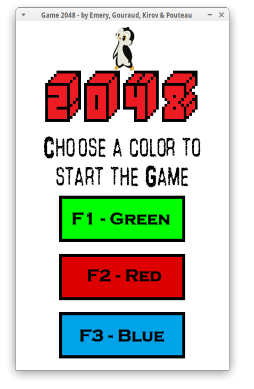
\includegraphics{screenshot-menu-jeu-sdl.png}
\end{figure}

\newpage
\subsection{Annexe 4 - Intelligence Artificielle}
\label{sec-7-4}
\noindent
Résultat de l'exécution de l'Intelligence Artificielle Rapide:
\begin{verbatim}
Sur 1000 lancés :

Nombre de fois 16 : 0
Nombre de fois 32 : 0
Nombre de fois 64 : 0
Nombre de fois 128 : 0
Nombre de fois 256 : 0
Nombre de fois 512 : 9
Nombre de fois 1024 : 81
Nombre de fois 2048 : 585
Nombre de fois 4096 : 322
Nombre de fois 8192 : 3
\end{verbatim}

\noindent
Résultat de l'exécution de l'Intelligence Artificielle Lente:
\begin{verbatim}
Sur 100 lancés : 

Nombre de fois 16 : 0
Nombre de fois 32 : 0
Nombre de fois 64 : 0
Nombre de fois 128 : 0
Nombre de fois 256 : 0
Nombre de fois 512 : 0
Nombre de fois 1024 : 5
Nombre de fois 2048 : 43
Nombre de fois 4096 : 51
Nombre de fois 8192 : 1
\end{verbatim}

\end{document}
